\documentclass{beamer}
\usepackage{parskip}

\setbeamertemplate{navigation symbols}{}

\usecolortheme{beaver}
\useinnertheme{circles}

\setbeamercolor{title}{bg=white}
\setbeamercolor{frametitle}{bg=white}

\setbeamertemplate{enumerate subitem}{\alph{enumii}.}

\renewcommand{\arraystretch}{1.25}

\graphicspath{{figures}}

\title{Midterm Review Tutorial}
\author{}
\date{}

\begin{document}

\begin{frame}
    \titlepage
\end{frame}

\begin{frame}{MIPS 21.8}
    \begin{center}
        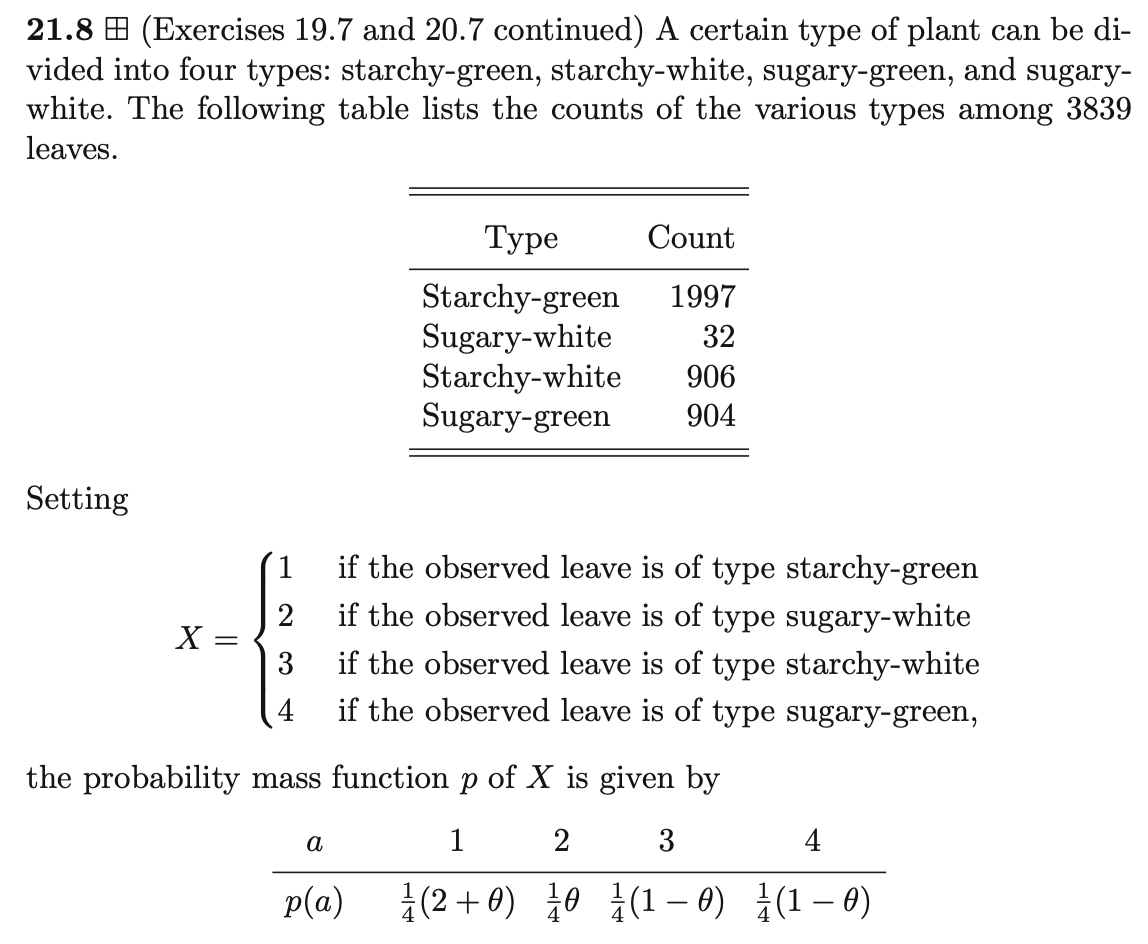
\includegraphics[width=0.61\textwidth]{MIPS_21.8_1.png}
        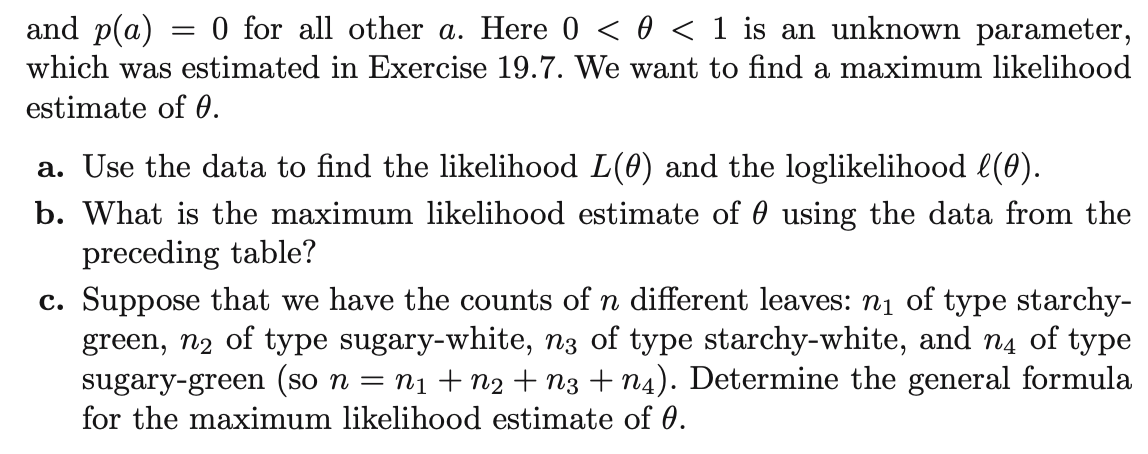
\includegraphics[width=0.61\textwidth]{MIPS_21.8_2.png}
    \end{center}
\end{frame}

\begin{frame}{MIPS 21.8 a}
    Use the data to find the likelihood $L(\theta)$ and the loglikelihood $\ell(\theta)$.
    \pause
    \begin{align*}
        \uncover<2->{L(\theta) &= \prod_{i=1}^{3839} p(x_i) \\}
        \uncover<3->{L(\theta) &= \left( \frac{2 + \theta}{4} \right)^{1997} \cdot \left( \frac{\theta}{4} \right)^{32} \cdot \left( \frac{1 - \theta}{4} \right)^{906} \cdot \left( \frac{1 - \theta}{4} \right)^{904} \\}
        \uncover<4->{L(\theta) &= \frac{1}{4^{3839}} \cdot (2 + \theta)^{1997} \cdot \theta^{32} \cdot (1 - \theta)^{1810} \\}
        \uncover<5->{\ell(\theta) &= -3839 \log(4) + 1997 \log(2 + \theta) + 32 \log(\theta) + 1810 \log(1 - \theta)}
    \end{align*}
\end{frame}

\begin{frame}{MIPS 21.8 b}
    What is the maximum likelihood estimate of $\theta$ using the data from the preceding table?
    \pause
    \begin{align*}
        \uncover<2->{\ell(\theta) &= -3839 \log(4) + 1997 \log(2 + \theta) + 32 \log(\theta) + 1810 \log(1 - \theta) \\}
        \uncover<3->{\ell'(\theta) &= \frac{1997}{2 + \theta} + \frac{32}{\theta} - \frac{1810}{1 - \theta} \\}
    \end{align*}
\end{frame}

\begin{frame}{MIPS 21.8 b}
    \begin{align*}
        \uncover<1->{0 &= \frac{1997}{2 + \hat{\theta}} + \frac{32}{\hat{\theta}} - \frac{1810}{1 - \hat{\theta}} \\}
        \uncover<2->{0 &= 1997\hat{\theta} \left( 1 - \hat{\theta} \right) + 32 \left( 2 + \hat{\theta} \right) \left( 1 - \hat{\theta} \right) - 1810\hat{\theta} \left( 2 + \hat{\theta} \right) \\}
        \uncover<3->{0 &= -3839\hat{\theta}^2 - 1655\hat{\theta} + 64 \\}
        \uncover<4->{&\cdots \\}
        \uncover<5->{\hat{\theta} &= \frac{1655 - \sqrt{3721809}}{-7678} \\}
        \uncover<6->{\hat{\theta} &\approx 0.0357}
    \end{align*}
\end{frame}

\begin{frame}{MIPS 21.8 c}
    Suppose that we have the counts of $n$ different leaves: $n_1$ of type starchy-green, $n_2$ of type sugary-white, $n_3$ of type starchy-white, and $n_4$ of type sugary-green (so $n = n_1 + n_2 + n_3 + n_4$). Determine the general formula for the maximum likelihood estimate of $\theta$.
\end{frame}

\begin{frame}{MIPS 21.8 c}
    \begin{align*}
        \uncover<1->{L(\theta) &= \prod_{i=1}^n p(x_i) \\}
        \uncover<2->{L(\theta) &= \left( \frac{2 + \theta}{4} \right)^{n_1} \cdot \left( \frac{\theta}{4} \right)^{n_2} \cdot \left( \frac{1 - \theta}{4} \right)^{n_3} \cdot \left( \frac{1 - \theta}{4} \right)^{n_4} \\}
        \uncover<3->{L(\theta) &= \frac{1}{4^n} \cdot (2 + \theta)^{n_1} \cdot \theta^{n_2} \cdot (1 - \theta)^{n_3 + n_4} \\}
        \uncover<4->{\ell(\theta) &= -n \log(4) + n_1 \log(2 + \theta) + n_2 \log(\theta) + (n_3 + n_4) \log(1 - \theta) \\}
        \uncover<5->{\ell'(\theta) &= \frac{n_1}{2 + \theta} + \frac{n_2}{\theta} - \frac{n_3 + n_4}{1 - \theta}}
    \end{align*}
\end{frame}

\begin{frame}{MIPS 21.8 c}
    \begin{align*}
        \uncover<1->{0 &= \frac{n_1}{2 + \hat{\theta}} + \frac{n_2}{\hat{\theta}} - \frac{n_3 + n_4}{1 - \hat{\theta}} \\}
        \uncover<2->{0 &= n_1\hat{\theta} \left( 1 - \hat{\theta} \right) + n_2 \left( 2 + \hat{\theta} \right) \left( 1 - \hat{\theta} \right) - (n_3 + n_4)\hat{\theta} \left( 2 + \hat{\theta} \right) \\}
        \uncover<3->{0 &= -n\hat{\theta}^2 + (n_1 - n_2 - 2n_3 - 2n_4)\hat{\theta} + 2n_2 \\}
        \uncover<4->{\hat{\theta} &= \frac{-n_1 + n_2 + 2n_3 + 2n_4 - \sqrt{(n_1 - n_2 - 2n_3 - 2n_4)^2 + 8nn_2}}{-2n}}
    \end{align*}
\end{frame}

\begin{frame}{Additional Problems}
    \begin{enumerate}
        \item Determine the method of moments estimator for $\theta$ using the first moment.
        \item Describe the empirical bootstrapping process for $B = 500$.
        \begin{enumerate}
            \item How many plants should you resample at each iteration?
        \end{enumerate}
        \item Describe the parametric bootstrapping process for $B = 500$.
        \begin{enumerate}
            \item How can you transform $U \sim \operatorname{Unif}(0, 1)$ to sample from $p(a)$?
        \end{enumerate}
        \item When would you choose empirical vs. parametric bootstrapping?
    \end{enumerate}
\end{frame}

\begin{frame}{Additional Problem 1}
    \begin{table}[h]
        \centering
        \begin{tabular}{c c c c c}
            $a$ & $1$ & $2$ & $3$ & $4$ \\
            \hline
            $p(a)$ & $\frac{1}{4} (2 + \theta)$ & $\frac{1}{4} \theta$ & $\frac{1}{4} (1 - \theta)$ & $\frac{1}{4} (1 - \theta)$ \\
        \end{tabular}
    \end{table}
    Determine the method of moments estimator for $\theta$ using the first moment.
    \pause
    \begin{align*}
       \uncover<2->{E[X] &= \sum_{x\in\{1, 2, 3, 4\}} x \cdot P(X = x) \\}
       \uncover<3->{E[X] &= \frac{2 + \theta}{4} + \frac{2\theta}{4} + \frac{3(1 - \theta)}{4} + \frac{4(1 - \theta)}{4} \\}
       \uncover<4->{E[X] &= \frac{9}{4} - \theta}
    \end{align*}
\end{frame}

\begin{frame}{Additional Problem 1}
    \begin{align*}
        \uncover<1->{\bar{X} &= \frac{9}{4} - \hat{\theta} \\}
        \uncover<2->{\hat{\theta} &= \frac{9}{4} - \bar{X}}
    \end{align*}
\end{frame}

\begin{frame}{Additional Problem 2}
    Describe the empirical bootstrapping process for $B = 500$.
    \pause
    
    Given a dataset $x_1, x_2, \dotsc, x_n$, determine its empirical distribution function $F_n$ as an estimate of $F$.
    \pause

    Compute the parameter
    \[
        \theta^* = \hat{\theta}
    \]
    (e.g., using MLE or MOM) corresponding to $F_n$.
\end{frame}

\begin{frame}{Additional Problem 2}
    Describe the empirical bootstrapping process for $B = 500$.
    \begin{enumerate}
        \item Generate a bootstrap dataset $x^*_1, x^*_2, \dotsc, x^*_n$ from $F_n$ (i.e., sample from the dataset with replacement).
        \pause
        \item Compute the estimate $\hat{\theta}^*$ of $\theta^* = \hat{\theta}$ (e.g., using MLE or MOM) for the bootstrap dataset.
        \pause
        \item Repeat steps 1 and 2 many times until you generate $B = 500$ bootstrapped estimates.
    \end{enumerate}
\end{frame}

\begin{frame}{Additional Problem 2a}
    How many plants should you resample at each iteration?
    \pause
    
    In the scenario from Exercise 21.8, you should resample $3839$ plants at each iteration since the sample size of the original dataset is $n = 3839$.
\end{frame}

\begin{frame}{Additional Problem 3}
    Describe the parametric bootstrapping process for $B = 500$.
    \pause

    Given a dataset $x_1, x_2, \dotsc, x_n$, compute an estimate $\hat{\theta}$ for $\theta$ (e.g., using MLE or MOM).
    \pause
    
    Determine $F_{\hat{\theta}}$ as an estimate for $F_\theta$, and use the parameter $\theta^* = \hat{\theta}$ corresponding to $F_{\hat{\theta}}$.
\end{frame}

\begin{frame}{Additional Problem 3}
    Describe the parametric bootstrapping process for $B = 500$.
    \begin{enumerate}
        \item Generate a bootstrap dataset $x^*_1, x^*_2, \dotsc, x^*_n$ from $F_{\hat{\theta}}$.
        \pause
        \item Compute the estimate $\hat{\theta}^*$ of $\theta^* = \hat{\theta}$ (e.g., using MLE or MOM) for the bootstrap dataset.
        \pause
        \item Repeat steps 1 and 2 many times until you generate $B = 500$ bootstrapped estimates.
    \end{enumerate}
\end{frame}

\begin{frame}{Additional Problem 3a}
    How can you transform $U \sim \operatorname{Unif}(0, 1)$ to sample from $p(a)$?
    \pause

    Suppose that the CDF of $X$ from Exercise 21.8 is $F$. We can use it to map probabilities back to the true percentiles of the distribution.
    \pause
    \begin{enumerate}
        \item Simulate a random sample of probabilities (i.e., randomly sample from the interval $[0, 1]$, which is the same as sampling from $\operatorname{Unif}(0, 1)$).
        \pause
        \item Transform the probabilities using $F^{-1}$.
        \pause
        \item The resulting values represent a random sample from the distribution $p(a)$ of $X$.
    \end{enumerate}
\end{frame}

\begin{frame}{Additional Problem 4}
    When would you choose empirical vs. parametric bootstrapping?
    \pause
    \begin{itemize}
        \item Use empirical bootstrapping when you are not certain about the model and want to test assumptions around a parametric model, or when you don't have any parametric model.
        \pause
        \item Use parametric bootstrapping when you are confident about the model, especially when the dataset is small and empirical resampling may not result in distributions representative of the population distribution.
    \end{itemize}
\end{frame}

\end{document}
